\chapter{The Business Process Modelling Notation}
\label{sec:bpmn}

%%% aus meiner Diplomarbeit

% introduction
The \emph{Business Process Modelling Notation}~\cite{omg2009bpmn} was first
published by the BPMI and has later been adopted by the OMG.  The goal of the
development of BPMN was to create a standardized modelling notation for business
processes and by that to reduce the confusion created by dozens of proprietary
business process notations.  A brief introduction to BPMN is given for instance
in~\cite{white2004introduction}.

% basic elements
There are four basic categories of element types in the notation: Flow Objects
(Events, Activities and Gateways), Connecting Objects (Sequence Flows, Message
Flows and Associations), Swimlanes (Pools and Lanes) and Artifacts (Data Objects,
Groups and Annotations).

\begin{figure}[ht]
	\centering
	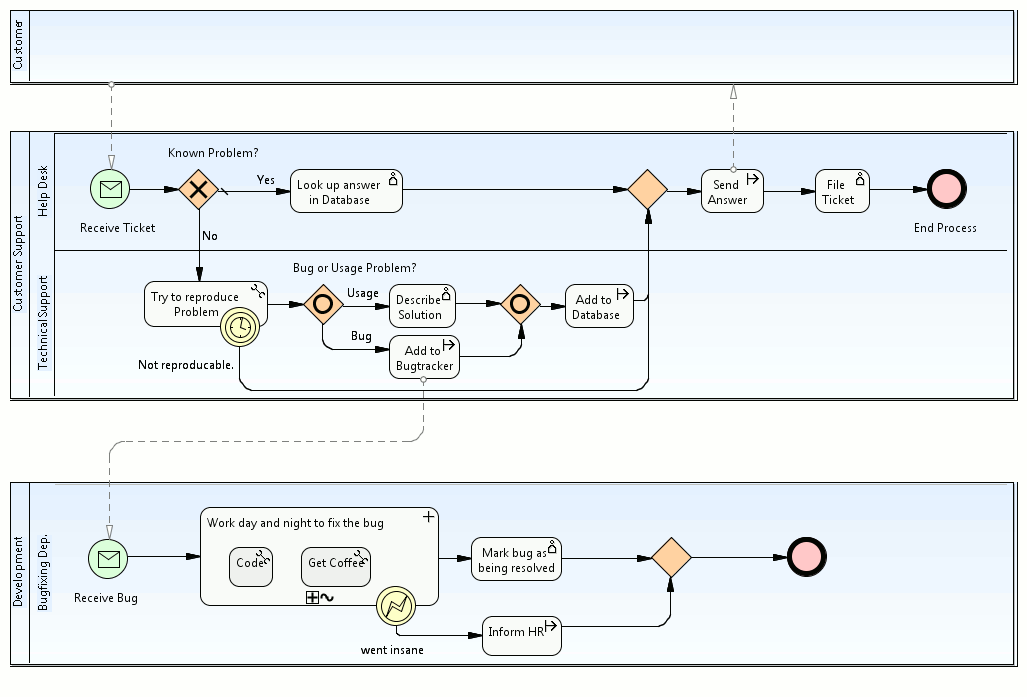
\includegraphics[width=.8\textwidth]{figures/bpmn/example.png}
	\caption{Business Process Modelling Notation Example Diagram}
	\label{fig:bpmn_example}
\end{figure}

Figure \ref{fig:bpmn_example} shows a simple example for an e-mail client
periodically looking for new mail.  The elements are quite self-descriptive and
most of them are already known from other notations, so the basics of the BPMN
are readily understandable for all business analysts, architects and developers
and even for non-experts.  At the same time BPMN provides a large variety of
subtypes for each of the Flow Objects and every element type is enriched with
many non-graphical attributes, making the models sufficiently detailed for being
exported to executable languages while keeping the visual notation concise and
understandable.

A problem with BPMN is that it is mainly a \emph{notation}.  Although the
specification describes many non-graphical attributes and a mapping to a formal
language, it neither states an exchange format, like an XSD, nor clear semantics
for all of the elements.  Still the Business Process Modelling Notation can be
used throughout the whole software engineering lifecycle, from a simplified model
at the requirements analysis up to a highly detailed model that can be used for
generating code for an executable language.


%%%%%%%%%%%%%%%%%%%%%%%%%%%%%%%%%%%%%%%%%%%%%%%%%%%%%%%%%%%%%%%%%%%%%%%%%%%%%%%%

\section{BPMN Elements}
\label{sec:bpmn_elements}

This section is intended to give a brief introduction of each of the basic element
groups:

\begin{itemize}
	\item \textbf{Flow Objects}: Events, Activities, and Gateways
	\item \textbf{Connecting Objects}: Sequence Flows, Message Flows and Associations
	\item \textbf{Swimlanes}: Pools and Lanes
	\item \textbf{Artifacts}: Data Objects, Groups and Annotations
\end{itemize}

\subsection{Flow Objects}

The category of \emph{Flow Objects}, the most important elements in BPMN, is made
up of \emph{Events}, \emph{Activities} and \emph{Gateways}.  All Flow Objects are
held in Lanes (see below).

\textbf{Events} are things that \emph{happen}, like a message arriving, an alarm,
or an error, and often they mark the beginning and the end of the process.  The
graphical notation is a circle.  They are subdivided into \emph{Start Events},
\emph{Intermediate Events} and \emph{End Events}, which will determine the circle's
border (see figure \ref{fig:events}).

\begin{figure}[ht]
	\centering
	
\includegraphics[width=.75\textwidth]{figures/bpmn/events.png}
	\caption[BPMN Event types]{BPMN Event types.  From left to right: Start Event,
	Intermediate Event, End Event}
	\label{fig:events}
\end{figure}

Further all three Event types have a variety of subtypes which will determine
e.g. a Start Event's \emph{trigger} and an end Event's \emph{result}.  Each of
these subtypes can be distinguished by a different icon in the centre of the Event
figure (see figure \ref{fig:triggers}) and results in a number of attributes to
be set for the Event.

\begin{figure}[ht]
	\centering
	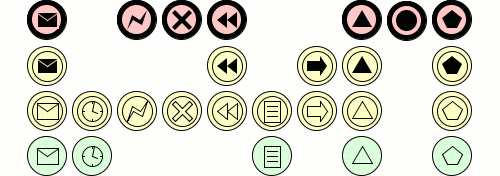
\includegraphics[width=.75\textwidth]{figures/bpmn/triggers.png}
	\caption[BPMN Event sub types]{BPMN Event sub types.  From left to right:
	Message, Timer, Error Cancel, Compensation, Rule, Link, Signal, Termination,
	Multiple}
	\label{fig:triggers}
\end{figure}

Basically, an \textbf{Activity} is something that is \emph{done}.  Activities
subdivide in \emph{Tasks}, which are atomic Activities, and \emph{Sub Processes},
which are composite Activities.  The graphical notation for an Activity is a
rounded rectangle with the Activity's name inside of it.  Sub Processes are marked
with a small $ \boxplus $ sign on the bottom line (see figure \ref{fig:activities}).

\begin{figure}[ht]
	\centering
	
\includegraphics[width=.75\textwidth]{figures/bpmn/activities.png}
	\caption[BPMN Activity types]{BPMN Activity types.  From left to right: Task,
	Subprocess}
	\label{fig:activities}
\end{figure}

Like Events, Activities also have some specializations, each one with special
attributes: They can be for instance a \emph{Send} or a \emph{Receive} Task, stand
for some \emph{Manual} work to be done, execute a \emph{Script} or, in case of
the \emph{Independent} Sub Process, represent a whole business process, just to
name a few.  All of these subtypes have the same graphical representation, but
modellers and modelling tools are free to extend the diagrams with additional
markers for the subtypes.

What makes Activities stand out from the other Flow Objects is that they can
\emph{loop}.  Although in BPMN loops also can be defined by simply connecting a
Sequence Flow to an upstream Flow Object, which might be easier to understand by
non-experts, it's seen as better style to use looping Sub Processes.  A looping
Activity is marked with a small counter-clockwise arrow on its bottom line.

\textbf{Gateways} provide wide capabilities in modelling all kinds of splitting
and merging behaviour.  Figure \ref{fig:gateways} shows the different kinds of
Gateways.  Depending on whether the Gateway has multiple incoming or outgoing
Sequence Flows -- or even both -- it has different semantics, like forking and/or
joining the flows.  However, Gateways are not the only way for modelling forking
and joining of flows.  In some cases the same semantics can be reached by omitting
the Gateway and connecting multiple Sequence Flows directly to an
Activity\footnote{this is not allowed for Events}.

\begin{figure}[ht]
	\centering
	
\includegraphics[width=.75\textwidth]{figures/bpmn/gateways.png}
	\caption[BPMN Gateway types]{BPMN Gateway types.  From left to right: Data
	based XOR (with and without marker), Event based XOR, Inclusive OR, Complex,
	AND}
	\label{fig:gateways}
\end{figure}


\subsection{Connecting Objects}

The most important connections are \emph{Sequence Flows} and \emph{Message Flows}.
Sequence Flows represent the flow of control and connect Flow Objects within a
Pool in the order of execution.  Message Flow represents messages -- not necessarily
data -- being exchanged exclusively between Pools.  See figure \ref{fig:connections}
for the connections' graphical notation.

\begin{figure}[ht]
	\centering
	
\includegraphics[width=.75\textwidth]{figures/bpmn/connections.png}
	\caption[BPMN Connection types]{BPMN Connection types.  From left to right:
	Sequence Flow, Message Flow, Association}
	\label{fig:connections}
\end{figure}

The third connection, the \emph{Association}, is mainly used for documentation
reason, for instance to connect a Text Annotation to a Flow Object that needs
further explanation.  Still there is an exception to this rule: For connecting a
compensating Activity to a compensation Event an Association is used instead of
a Sequence Flow.  An Association's arrow heads are optional.


\subsection{Swimlanes}

Swimlanes can be \emph{Pools} and \emph{Lanes}.  Each Pool represents one
Participant in the business process, while Lanes are used to partition a Pool.
Doing so each of a company's departments could be represented by a Lane while the
Pool stands for the company itself.  Typically Pools and Lanes are oriented
horizontally, but they may be oriented vertically, too.  Further, Lanes may cross
or contain other Lanes, but those techniques are poorly documented and usually
not used.  Figure \ref{fig:swimlanes} shows a small horizontally oriented Pool
containing two empty Lanes.

\begin{figure}[ht]
	\centering
	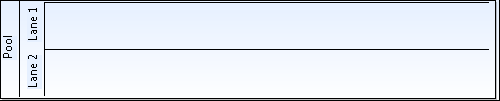
\includegraphics[width=.75\textwidth]{figures/bpmn/swimlanes.png}
	\caption[BPMN Swimlanes]{BPMN Swimlanes. A Pool with two Lanes}
	\label{fig:swimlanes}
\end{figure}


\subsection{Artifacts}

The main purpose of \emph{Artifacts} is documentation.  However, like Associations,
in some situations they can have semantics, e.g. when a \emph{Data Object} is
referenced by an Activity as input.  Data Objects represent everything that can
be input or output of some Activity.  In most cases this will be a file, but since
Activities can be \emph{Manual Tasks}, too, a Data Object could also stand for
something physical.

The other two Artifacts, \emph{Group} and \emph{Text Annotation}, are solely used
for documentation.  See figure \ref{fig:artifacts} for their graphical notation.

\begin{figure}[ht]
	\centering
	
\includegraphics[width=.75\textwidth]{figures/bpmn/artifacts.png}
	\caption[BPMN Artifacts]{BPMN Artifacts.  From left to right: Data Object,
	Group, Text Annotation}
	\label{fig:artifacts}
\end{figure}

The specification states that this category may be extended by proprietary
Artifacts which could have more semantics, too.  This way BPMN can be extended
with new elements to represent concepts that were not considered in the original
specification.


%%%%%%%%%%%%%%%%%%%%%%%%%%%%%%%%%%%%%%%%%%%%%%%%%%%%%%%%%%%%%%%%%%%%%%%%%%%%%%%%

\section{Levels of Complexity}
\label{sec:bpmn_complexity}

% drei layer
BPMN can be seen as having at least three levels of complexity.

\begin{enumerate}
	\item Basic Types: All diagrams are made up of the basic elements of the four
	categories: Events, Activities, Gateways, Connections, Pools and Artifacts.
	These can be understood easily even by non-experts.
	
	\item Subtypes: The Flow Objects each have several subtypes, e.g.  Timer
	Events, Receive Tasks and Inclusive Gateways.  Using the same shapes as the
	basic elements enriched with some additional graphical information, like an
	icon, the symbol's basic type can be clearly identified by non-experts while
	providing additional visual information for the professionals.
	
	\item Attributes: Each of the BPMN element types provides a large number of
	both primitive and complex attributes.  While some of these attributes are
	visible in the diagram, like a flow object's name or subtype, most are
	non-graphical.  These attributes enrich the diagram with the formal semantics
	necessary for the export to an executable language while not polluting the
	visual notation with too many details.
\end{enumerate}

% notation teils ohne semantik (message flows)
If the process shall be mapped to a executable language the third level is very
important: Not only does it give values for many attributes that otherwise would
have to be set manually.  Some of the visual elements of the BPMN do not have
semantics ``on their own''.  Message Flows for example do \emph{not} have a
mapping to WS-BPEL.  Instead the source Activity has to be of type \texttt{Send}
and the target Activity of type \texttt{Receive}, and both have to reference the
same non-graphical \texttt{Message} element.  This is necessary in cases when the
communications partner is not in the same diagram and thus a Message Flow can not
be drawn.

Of course it is free to the designers of new mappings to map the Message Flow, if
it is available, without insisting on the existence of the non-graphical Message
element.


%%%%%%%%%%%%%%%%%%%%%%%%%%%%%%%%%%%%%%%%%%%%%%%%%%%%%%%%%%%%%%%%%%%%%%%%%%%%%%%%

\section{Export and Code Generation}
\label{sec:bpmn_export}

One of the main purposes of the Business Process Modelling Notation is to provide
a graphical notation that can be used to generate executable code from it.

A mapping to WS-BPEL is given in the BPMN Specification.  As a matter of fact,
BPMN has been tailored for the mapping to WS-BPEL, which can be seen in many
attributes which are needed only for the mapping.  Most of these attributes can
be reused for mappings to other languages, too, e.g. such common concepts as
properties and assignments.

On the other hand BPMN has more expressive power than BPEL.  A diagram in BPMN is
a directed graph, while BPEL, and in fact most other executive languages as well,
are block oriented, making the export to a semantically equivalent program
complicated and in some cases impossible.  Numerous papers have been written on
how to identify block structures within a BPMN diagram or how to alter an existing
diagram to conform to block structure.  However, not every diagram can be
refactored like that.

While the basic elements such as Flow Objects should neither be altered nor
extended by new elements the BPMN Specification encourages the introduction of
new, domain-specific Artifacts to be used in mappings to executable languages
other than BPEL.  These elements can be associated with the original BPMN elements
and represent concepts that were not considered in the original BPMN specification.

